\documentclass{article}
\usepackage{luatextra}
\usepackage{polyglossia}
\usepackage{ulem}
\usepackage{framed}
\usepackage{color}
\usepackage{geometry}
\usepackage{amsmath}
\usepackage{unicode-math}
\usepackage[hidelinks]{hyperref}
\usepackage{latexsym}
\usepackage{pdflscape}
\usepackage{pdfpages}
\usepackage{enumitem}
\usepackage{titlesec}
\usepackage{lastpage}
\usepackage{fancyhdr}
\usepackage{titlesec}
\usepackage{listings}
\usepackage{graphicx}

\usepackage{ifluatex}
\ifluatex
  \usepackage{pdftexcmds}
  \makeatletter
  \let\pdfstrcmp\pdf@strcmp
  \let\pdffilemoddate\pdf@filemoddate
  \makeatother
\fi
\usepackage{svg}

\setmathfont{xits-math.otf}

\setmainlanguage{french}
\selectlanguage{french}
%%\setmainfont{Latin Modern Roman}
\setmainfont{Roboto}

\geometry{margin={1in,1in}}

\setlist{nosep} %% No space between lists' items

\pagestyle{fancy}
\fancyhead[R]{}

%% <current page>/<total pages> footer
\cfoot{\thepage/\pageref{LastPage}}

\newcommand\image[2]{
\directlua{
local image = img.scan({filename = "#1"})

image.height = image.height * #2
image.width  = image.width  * #2

node.write(img.node(image))
}
}


%%%%%%%%%%%%%%%%%%%%%%%%%%%%%%%%%%%%%%%%%%
%% \subsubsubsection command definition %%
%%%%%%%%%%%%%%%%%%%%%%%%%%%%%%%%%%%%%%%%%%


\titleclass{\subsubsubsection}{straight}[\subsection]

\newcounter{subsubsubsection}[subsubsection]
\renewcommand\thesubsubsubsection{\thesubsubsection.\arabic{subsubsubsection}}
\renewcommand\theparagraph{\thesubsubsubsection.\arabic{paragraph}} % optional; useful if paragraphs are to be numbered

\titleformat{\subsubsubsection}
  {\normalfont\normalsize\bfseries}{\thesubsubsubsection}{1em}{}
\titlespacing*{\subsubsubsection}
{0pt}{3.25ex plus 1ex minus .2ex}{1.5ex plus .2ex}

\makeatletter
\renewcommand\paragraph{\@startsection{paragraph}{5}{\z@}%
  {3.25ex \@plus1ex \@minus.2ex}%
  {-1em}%
  {\normalfont\normalsize\bfseries}}
\renewcommand\subparagraph{\@startsection{subparagraph}{6}{\parindent}%
  {3.25ex \@plus1ex \@minus .2ex}%
  {-1em}%
  {\normalfont\normalsize\bfseries}}
\def\toclevel@subsubsubsection{4}
\def\toclevel@paragraph{5}
\def\toclevel@paragraph{6}
\def\l@subsubsubsection{\@dottedtocline{4}{7em}{4em}}
\def\l@paragraph{\@dottedtocline{5}{10em}{5em}}
\def\l@subparagraph{\@dottedtocline{6}{14em}{6em}}
\makeatother

\setcounter{secnumdepth}{4}
\setcounter{tocdepth}{4}

%%%%%%%%%%%%%%%%%%%%%%%%%%%%%%%%%%%%%%%%%%
%% end \subsubsubsection definition     %%
%%%%%%%%%%%%%%%%%%%%%%%%%%%%%%%%%%%%%%%%%%


\titlespacing*{\section}{0pt}{0.7\baselineskip}{0.7\baselineskip}

\title{Projet Principe d'éxécution des programmes}
%\subtitle{Meow}
\author{NassimBounouas, piernov}
\date{\today}

\begin{document}
\lstset{xleftmargin=.25in}

\maketitle
\textcolor{blue}{\url{https://github.com/NassimBounouas/Stage_SI3_PeP}}
\tableofcontents

\newpage

\section{Présentation du projet}
\subsection{Le microprocesseur ARM Cortex-M0}
	Le microprocesseur ARM Cortex-M0 

\subsection{Assembleur}

\subsubsection{Syntaxe}
Syntaxe UAL\\
S: màj des drapeaux\\
<c>: condition\\
Rd: registre destination\\
<imm?>: immédiat\\
SP: registre de pointeur de pile en mémoire\\
opcode: code de l'instruction, peut occuper jusqu'à la taille indiquée\\
\[\]: argument optionnel\\

\section{Jeu d'instructions (Instruction Set Architecture)}

\subsection{Instructions à implémenter}

\textbf{Binaire:}\\

\begin{tabular}{| c c c c c c c c c c c c c c c c |}
\hline
15 & 14 & 13 & 12 & 11 & 10 & \multicolumn{1}{|c}{9} & 8 & 7 & 6 & 5 & 4 & 3 & 2 & 1 & 0 \\
\hline
\multicolumn{6}{|c}{opcode} & \multicolumn{10}{|c|}{} \\
\hline
\end{tabular}


\subsubsection{Shift, add, sub, mov}

\textbf{Binaire:}\\

\begin{tabular}{| c c c c c c c c c c c c c c c c |}
\hline
15 & 14 & \multicolumn{1}{|c}{13} & 12 & 11 & 10 & 9 & \multicolumn{1}{|c}{8} & 7 & 6 & 5 & 4 & 3 & 2 & 1 & 0 \\
\hline
0 & 0 & \multicolumn{5}{|c}{opcode} & \multicolumn{9}{|c|}{} \\
\hline
\end{tabular}


\subsubsubsection{LSL (immediate): Logical Shift Left (p. 298)}

\textbf{Description: }

Décale le contenu du registre \texttt{Rm} vers la gauche d'un nombre de bits donné par l'immédiat \texttt{imm5}, écrit le résultat dans le registre \texttt{Rd}.\\
Des zéros sont insérés à droite.\\
Les drapeaux sont mis à jour.\\

\textbf{Assembleur:} T1

\begin{lstlisting}
LSLS <Rd>,<Rm>,#<imm5>
\end{lstlisting}

\textbf{Binaire:}\\

\begin{tabular}{| c c c c c c c c c c c c c c c c |}
\hline
15 & 14 & 13 & \multicolumn{1}{|c}{12} & 11 & \multicolumn{1}{|c}{10} & 9 & 8 & 7 & 6 & \multicolumn{1}{|c}{5} & 4 & 3 & \multicolumn{1}{|c}{2} & 1 & 0 \\
\hline
0 & 0 & 0 & \multicolumn{1}{|c}{0} & 0 & \multicolumn{5}{|c|}{imm5} & \multicolumn{3}{|c|}{Rm} & \multicolumn{3}{|c|}{Rd} \\
\hline
\end{tabular}

\subsubsubsection{LSR (immediate): Logical Shift Right (p. 302)}

\textbf{Description: }

Décale le contenu du registre \texttt{Rm} vers la droite d'un nombre de bits donné par l'immédiat \texttt{imm5}, écrit le résultat dans le registre \texttt{Rd}.\\
Des zéros sont insérés à gauche.\\
Les drapeaux sont mis à jour.\\

\textbf{Assembleur:} T1

\begin{lstlisting}
LSRS <Rd>,<Rm>,#<imm5>
\end{lstlisting}

\textbf{Binaire:}\\

\begin{tabular}{| c c c c c c c c c c c c c c c c |}
\hline
15 & 14 & 13 & \multicolumn{1}{|c}{12} & 11 & \multicolumn{1}{|c}{10} & 9 & 8 & 7 & 6 & \multicolumn{1}{|c}{5} & 4 & 3 & \multicolumn{1}{|c}{2} & 1 & 0 \\
\hline   
0 & 0 & 0 & \multicolumn{1}{|c}{0} & 1 & \multicolumn{5}{|c|}{imm5} & \multicolumn{3}{|c|}{Rm} & \multicolumn{3}{|c|}{Rd} \\
\hline
\end{tabular}


\subsubsubsection{ASR (immediate): Arithmetic Shift Right (p. 203)}

\textbf{Description: }

Décale le contenu du registre \texttt{Rm} vers la droite d'un nombre de bits donné par l'immédiat \texttt{imm5}, écrit le résultat dans le registre \texttt{Rd}.\\
Le bit de signe de \texttt{Rm} est ré-inséré à gauche.\\
Les drapeaux sont mis à jour.\\

\textbf{Assembleur:} T1

\begin{lstlisting}
ASRS <Rd>,<Rm>,#<imm5>
\end{lstlisting}

\textbf{Binaire:}\\

\begin{tabular}{| c c c c c c c c c c c c c c c c |}
\hline
15 & 14 & 13 & \multicolumn{1}{|c}{12} & 11 & \multicolumn{1}{|c}{10} & 9 & 8 & 7 & 6 & \multicolumn{1}{|c}{5} & 4 & 3 & \multicolumn{1}{|c}{2} & 1 & 0 \\
\hline   
0 & 0 & 0 & \multicolumn{1}{|c}{1} & 0 & \multicolumn{5}{|c|}{imm5} & \multicolumn{3}{|c|}{Rm} & \multicolumn{3}{|c|}{Rd} \\
\hline
\end{tabular}


\subsubsubsection{ADD (register): Add register (p. 191)}

\textbf{Description: }

Ajoute le contenu du registre \texttt{Rn} au contenu du registre \texttt{Rm}, écrit le résultat dans le registre \texttt{Rd}.\\
Les drapeaux sont mis à jour.\\

\textbf{Assembleur:} T1

\begin{lstlisting}
ADDS <Rd>,<Rn>,<Rm>
\end{lstlisting}

\textbf{Binaire:}\\

\begin{tabular}{| c c c c c c c c c c c c c c c c |}
\hline
15 & 14 & 13 & \multicolumn{1}{|c}{12} & 11 & \multicolumn{1}{|c}{10} & \multicolumn{1}{|c}{9} & \multicolumn{1}{|c}{8} & 7 & 6 & \multicolumn{1}{|c}{5} & 4 & 3 & \multicolumn{1}{|c}{2} & 1 & 0 \\
\hline   
0 & 0 & 0 & \multicolumn{1}{|c}{1} & 1 &  \multicolumn{1}{|c}{0} & \multicolumn{1}{|c}{0} & \multicolumn{3}{|c|}{Rm} & \multicolumn{3}{|c|}{Rn} & \multicolumn{3}{|c|}{Rd} \\
\hline
\end{tabular}


\subsubsubsection{SUB (register): Substract register (p. 450)}

\textbf{Description: }
Soustrait le contenu du registre \texttt{Rn} au contenu du registre \texttt{Rm}, écrit le résultat dans le registre \texttt{Rd}.\\
Les drapeaux sont mis à jour.\\

\textbf{Assembleur:} T1

\begin{lstlisting}
SUBS <Rd>,<Rn>,<Rm>
\end{lstlisting}

\textbf{Binaire:}\\

\begin{tabular}{| c c c c c c c c c c c c c c c c |}
\hline
15 & 14 & 13 & \multicolumn{1}{|c}{12} & 11 & \multicolumn{1}{|c}{10} & \multicolumn{1}{|c}{9} & \multicolumn{1}{|c}{8} & 7 & 6 & \multicolumn{1}{|c}{5} & 4 & 3 & \multicolumn{1}{|c}{2} & 1 & 0 \\
\hline   
0 & 0 & 0 & \multicolumn{1}{|c}{1} & 1 &  \multicolumn{1}{|c}{0} & \multicolumn{1}{|c}{1} & \multicolumn{3}{|c|}{Rm} & \multicolumn{3}{|c|}{Rn} & \multicolumn{3}{|c|}{Rd} \\
\hline
\end{tabular}

\subsubsubsection{MOV (immediate): Move (p. 312)}

\textbf{Description: }

Écrit l'immédiat \texttt{imm8} dans le registre \texttt{Rd}.\\
Les drapeaux sont mis à jour.\\

\textbf{Assembleur:} T1

\begin{lstlisting}
MOVS <Rd>,#<imm8>
\end{lstlisting}

\textbf{Binaire:}\\

\begin{tabular}{| c c c c c c c c c c c c c c c c |}
\hline
15 & 14 & 13 & \multicolumn{1}{|c}{12} & 11 & \multicolumn{1}{|c}{10} & 9 & 8 & \multicolumn{1}{|c}{7} & 6 & 5 & 4 & 3 & 2 & 1 & 0 \\
\hline
0 & 0 & 1 & \multicolumn{1}{|c}{0} & 0 & \multicolumn{3}{|c|}{Rd} & \multicolumn{8}{|c|}{imm8} \\
\hline
\end{tabular}


\subsubsection{Data processing}

\textbf{Binaire:}\\

\begin{tabular}{| c c c c c c c c c c c c c c c c |}
\hline
15 & 14 & 13 & 12 & 11 & 10 & \multicolumn{1}{|c}{9} & 8 & 7 & 6 & \multicolumn{1}{|c}{5} & 4 & 3 & 2 & 1 & 0 \\
\hline
0 & 1 & 0 & 0 & 0 & 0 & \multicolumn{4}{|c}{opcode} & \multicolumn{6}{|c|}{} \\
\hline
\end{tabular}

\subsubsubsection{AND (register): Bitwise AND (p. 201)}

\textbf{Description: }

Effectue un ET binaire entre le contenu du registre \texttt{Rdn} et le contenu du registre \texttt{Rm}, écrit le résultat dans le registre \texttt{Rdn}.\\
Les drapeaux sont mis à jour.\\

\textbf{Assembleur:} T1

\begin{lstlisting}
ANDS <Rdn>,<Rm>
\end{lstlisting}

\textbf{Binaire:}\\

\begin{tabular}{| c c c c c c c c c c c c c c c c |}
\hline
15 & 14 & 13 & 12 & 11 & 10 & \multicolumn{1}{|c}{9} & 8 & 7 & 6 & \multicolumn{1}{|c}{5} & 4 & 3 & \multicolumn{1}{|c}{2} & 1 & 0 \\
\hline
0 & 1 & 0 & 0 & 0 & 0 & \multicolumn{1}{|c}{0} & 0 & 0 & 0 & \multicolumn{3}{|c}{Rm} & \multicolumn{3}{|c|}{Rdn} \\
\hline
\end{tabular}


\subsubsubsection{EOR (register): Exclusive OR (p. 239)}

\textbf{Description: }

Effectue un OU exclusif binaire entre le contenu du registre \texttt{Rdn} et le contenu du registre \texttt{Rm}, écrit le résultat dans le registre \texttt{Rdn}.\\
Les drapeaux sont mis à jour.\\

\textbf{Assembleur:} T1

\begin{lstlisting}
EORS <Rdn>,<Rm>
\end{lstlisting}

\textbf{Binaire:}\\

\begin{tabular}{| c c c c c c c c c c c c c c c c |}
\hline
15 & 14 & 13 & 12 & 11 & 10 & \multicolumn{1}{|c}{9} & 8 & 7 & 6 & \multicolumn{1}{|c}{5} & 4 & 3 & \multicolumn{1}{|c}{2} & 1 & 0 \\
\hline
0 & 1 & 0 & 0 & 0 & 0 & \multicolumn{1}{|c}{0} & 0 & 0 & 1 & \multicolumn{3}{|c}{Rm} & \multicolumn{3}{|c|}{Rdn} \\
\hline
\end{tabular}


\subsubsubsection{LSL (register): Logical Shift Left (p. 300)}

\textbf{Description: }

Décale le contenu du registre \texttt{Rdn} vers la gauche d'un nombre de bits donné par l'octet inférieur du registre \texttt{Rm}, écrit le résultat dans le registre \texttt{Rdn}.\\
Des zéros sont insérés à droite.\\
Les drapeaux sont mis à jour.\\

\textbf{Assembleur:} T1

\begin{lstlisting}
LSLS <Rdn>,<Rm>
\end{lstlisting}

\textbf{Binaire:}\\

\begin{tabular}{| c c c c c c c c c c c c c c c c |}
\hline
15 & 14 & 13 & 12 & 11 & 10 & \multicolumn{1}{|c}{9} & 8 & 7 & 6 & \multicolumn{1}{|c}{5} & 4 & 3 & \multicolumn{1}{|c}{2} & 1 & 0 \\
\hline
0 & 1 & 0 & 0 & 0 & 0 & \multicolumn{1}{|c}{0} & 0 & 1 & 0 & \multicolumn{3}{|c}{Rm} & \multicolumn{3}{|c|}{Rdn} \\
\hline
\end{tabular}



\subsubsubsection{LSR (register): Logical Shift Right (p. 304)}

\textbf{Description: }

Décale le contenu du registre \texttt{Rdn} vers la droite d'un nombre de bits donné par l'octet inférieur du registre \texttt{Rm}, écrit le résultat dans le registre \texttt{Rdn}.\\
Des zéros sont insérés à gauche.\\
Les drapeaux sont mis à jour.\\

\textbf{Assembleur:} T1

\begin{lstlisting}
LSRS <Rdn>,<Rm>
\end{lstlisting}

\textbf{Binaire:}\\

\begin{tabular}{| c c c c c c c c c c c c c c c c |}
\hline
15 & 14 & 13 & 12 & 11 & 10 & \multicolumn{1}{|c}{9} & 8 & 7 & 6 & \multicolumn{1}{|c}{5} & 4 & 3 & \multicolumn{1}{|c}{2} & 1 & 0 \\
\hline
0 & 1 & 0 & 0 & 0 & 0 & \multicolumn{1}{|c}{0} & 0 & 1 & 1 & \multicolumn{3}{|c}{Rm} & \multicolumn{3}{|c|}{Rdn} \\
\hline
\end{tabular}


\subsubsubsection{ASR (register): Arithmetic Shift Right (p. 205)}

\textbf{Description: }

Décale le contenu du registre \texttt{Rdn} vers la droite d'un nombre de bits donné par l'octet inférieur du registre \texttt{Rm}, écrit le résultat dans le registre \texttt{Rdn}.\\
Le bit de signe de \texttt{Rdn} est ré-inséré à gauche.\\
Les drapeaux sont mis à jour.\\

\textbf{Assembleur:} T1

\begin{lstlisting}
ASRS <Rdn>,<Rm>
\end{lstlisting}

\textbf{Binaire:}\\

\begin{tabular}{| c c c c c c c c c c c c c c c c |}
\hline
15 & 14 & 13 & 12 & 11 & 10 & \multicolumn{1}{|c}{9} & 8 & 7 & 6 & \multicolumn{1}{|c}{5} & 4 & 3 & \multicolumn{1}{|c}{2} & 1 & 0 \\
\hline
0 & 1 & 0 & 0 & 0 & 0 & \multicolumn{1}{|c}{0} & 1 & 0 & 0 & \multicolumn{3}{|c}{Rm} & \multicolumn{3}{|c|}{Rdn} \\
\hline
\end{tabular}


\subsubsubsection{ADC (register): Add with Carry (p. 187)}

\textbf{Description: }

Ajoute le contenu du registre \texttt{Rm} et le drapeau de retenu au contenu du registre \texttt{Rdn}, écrit le résultat dans le registre \texttt{Rdn}.\\
Les drapeaux sont mis à jour.\\

\textbf{Assembleur:} T1

\begin{lstlisting}
ADCS <Rdn>,<Rm>
\end{lstlisting}

\textbf{Binaire:}\\

\begin{tabular}{| c c c c c c c c c c c c c c c c |}
\hline
15 & 14 & 13 & 12 & 11 & 10 & \multicolumn{1}{|c}{9} & 8 & 7 & 6 & \multicolumn{1}{|c}{5} & 4 & 3 & \multicolumn{1}{|c}{2} & 1 & 0 \\
\hline
0 & 1 & 0 & 0 & 0 & 0 & \multicolumn{1}{|c}{0} & 1 & 0 & 1 & \multicolumn{3}{|c}{Rm} & \multicolumn{3}{|c|}{Rdn} \\
\hline
\end{tabular}

\subsubsubsection{SBC (register): Substract with Carry (p. 380)}

\textbf{Description: }

Soustrait le contenu du registre \texttt{Rm} et le complément du drapeau de retenu au contenu du registre \texttt{Rdn}, écrit le résultat dans le registre \texttt{Rdn}.\\
Les drapeaux sont mis à jour.\\

\textbf{Assembleur:} T1

\begin{lstlisting}
SBCS <Rdn>,<Rm>
\end{lstlisting}

\textbf{Binaire:}\\

\begin{tabular}{| c c c c c c c c c c c c c c c c |}
\hline
15 & 14 & 13 & 12 & 11 & 10 & \multicolumn{1}{|c}{9} & 8 & 7 & 6 & \multicolumn{1}{|c}{5} & 4 & 3 & \multicolumn{1}{|c}{2} & 1 & 0 \\
\hline
0 & 1 & 0 & 0 & 0 & 0 & \multicolumn{1}{|c}{0} & 1 & 1 & 0 & \multicolumn{3}{|c}{Rm} & \multicolumn{3}{|c|}{Rdn} \\
\hline
\end{tabular}



\subsubsubsection{ROR (register): Rotate Right (p. 368)}

\textbf{Description: }

Pivote le contenu du registre \texttt{Rdn} vers la droite d'un nombre de bits donné par l'octet inférieur du registre \texttt{Rm}, écrit le résultat dans le registre \texttt{Rdn}.\\
Les bits de \texttt{Rdn} sortant à droite sont ré-insérés à gauche.\\
Les drapeaux sont mis à jour.\\

\textbf{Assembleur:} T1

\begin{lstlisting}
RORS <Rdn>,<Rm>
\end{lstlisting}

\textbf{Binaire:}\\

\begin{tabular}{| c c c c c c c c c c c c c c c c |}
\hline
15 & 14 & 13 & 12 & 11 & 10 & \multicolumn{1}{|c}{9} & 8 & 7 & 6 & \multicolumn{1}{|c}{5} & 4 & 3 & \multicolumn{1}{|c}{2} & 1 & 0 \\
\hline
0 & 1 & 0 & 0 & 0 & 0 & \multicolumn{1}{|c}{0} & 1 & 1 & 1 & \multicolumn{3}{|c}{Rm} & \multicolumn{3}{|c|}{Rdn} \\
\hline
\end{tabular}


\subsubsubsection{TST (register): Set flags on bitwise AND (p. 466)}

\textbf{Description: }

Effectue un ET logique entre le contenu du registre \texttt{Rn} et le contenu du registre \texttt{Rm}, le résultat n'est pas écrit.\\
Les drapeaux sont mis à jour.\\

\textbf{Assembleur:} T1

\begin{lstlisting}
TST <Rn>,<Rm>
\end{lstlisting}

\textbf{Binaire:}\\

\begin{tabular}{| c c c c c c c c c c c c c c c c |}
\hline
15 & 14 & 13 & 12 & 11 & 10 & \multicolumn{1}{|c}{9} & 8 & 7 & 6 & \multicolumn{1}{|c}{5} & 4 & 3 & \multicolumn{1}{|c}{2} & 1 & 0 \\
\hline
0 & 1 & 0 & 0 & 0 & 0 & \multicolumn{1}{|c}{1} & 0 & 0 & 0 & \multicolumn{3}{|c}{Rm} & \multicolumn{3}{|c|}{Rn} \\
\hline
\end{tabular}



\subsubsubsection{RSB (immediate): Reverse Substract from 0 (p. 372)}

\textbf{Description: }

Soustrait le contenu du registre \texttt{Rn} à l'immédiat 0, écrit le résultat dans le registre \texttt{Rd}.\\
Les drapeaux sont mis à jour.\\

\textbf{Assembleur:} T1

\begin{lstlisting}
RSBS <Rd>,<Rn>,#0
\end{lstlisting}

\textbf{Binaire:}\\

\begin{tabular}{| c c c c c c c c c c c c c c c c |}
\hline
15 & 14 & 13 & 12 & 11 & 10 & \multicolumn{1}{|c}{9} & 8 & 7 & 6 & \multicolumn{1}{|c}{5} & 4 & 3 & \multicolumn{1}{|c}{2} & 1 & 0 \\
\hline
0 & 1 & 0 & 0 & 0 & 0 & \multicolumn{1}{|c}{1} & 0 & 0 & 1 & \multicolumn{3}{|c}{Rn} & \multicolumn{3}{|c|}{Rd} \\
\hline
\end{tabular}



\subsubsubsection{CMP (register): Compare Registers (p. 231)}

\textbf{Description: }

Soustrait le contenu du registre \texttt{Rm} au contenu du registre \texttt{Rn}, le résultat n'est pas écrit.\\
Les drapeaux sont mis à jour.\\

\textbf{Assembleur:} T1

\begin{lstlisting}
CMP <Rn>,<Rm>
\end{lstlisting}

\textbf{Binaire:}\\

\begin{tabular}{| c c c c c c c c c c c c c c c c |}
\hline
15 & 14 & 13 & 12 & 11 & 10 & \multicolumn{1}{|c}{9} & 8 & 7 & 6 & \multicolumn{1}{|c}{5} & 4 & 3 & \multicolumn{1}{|c}{2} & 1 & 0 \\
\hline
0 & 1 & 0 & 0 & 0 & 0 & \multicolumn{1}{|c}{1} & 0 & 1 & 0 & \multicolumn{3}{|c}{Rm} & \multicolumn{3}{|c|}{Rn} \\
\hline
\end{tabular}


\subsubsubsection{CMN (register): Compare Negative (p. 227)}

\textbf{Description: }

Ajoute le contenu du registre \texttt{Rm} au contenu du registre \texttt{Rn}, le résultat n'est pas écrit.\\
Les drapeaux sont mis à jour.\\

\textbf{Assembleur:} T1

\begin{lstlisting}
CMN <Rn>,<Rm>
\end{lstlisting}

\textbf{Binaire:}\\

\begin{tabular}{| c c c c c c c c c c c c c c c c |}
\hline
15 & 14 & 13 & 12 & 11 & 10 & \multicolumn{1}{|c}{9} & 8 & 7 & 6 & \multicolumn{1}{|c}{5} & 4 & 3 & \multicolumn{1}{|c}{2} & 1 & 0 \\
\hline
0 & 1 & 0 & 0 & 0 & 0 & \multicolumn{1}{|c}{1} & 0 & 1 & 1 & \multicolumn{3}{|c}{Rm} & \multicolumn{3}{|c|}{Rn} \\
\hline
\end{tabular}


\subsubsubsection{ORR (register): Logical OR (p. 336)}

\textbf{Description: }

Effectue un OU binaire entre le contenu du registre \texttt{Rdn} et le contenu du registre \texttt{Rm}, écrit le résultat dans le registre \texttt{Rdn}.\\
Les drapeaux sont mis à jour.\\

\textbf{Assembleur:} T1

\begin{lstlisting}
ORRS <Rdn>,<Rm>
\end{lstlisting}

\textbf{Binaire:}\\

\begin{tabular}{| c c c c c c c c c c c c c c c c |}
\hline
15 & 14 & 13 & 12 & 11 & 10 & \multicolumn{1}{|c}{9} & 8 & 7 & 6 & \multicolumn{1}{|c}{5} & 4 & 3 & \multicolumn{1}{|c}{2} & 1 & 0 \\
\hline
0 & 1 & 0 & 0 & 0 & 0 & \multicolumn{1}{|c}{1} & 1 & 0 & 0 & \multicolumn{3}{|c}{Rm} & \multicolumn{3}{|c|}{Rdn} \\
\hline
\end{tabular}


\subsubsubsection{MUL: Multiply Two Registers (p. 324)}

\textbf{Description: }

Multiplie le contenu du registre \texttt{Rn} avec le contenu du registre \texttt{Rdm}, écrit les 32 bits de poids faible du résultat dans le registre \texttt{Rdm}.\\
Les drapeaux sont mis à jour.\\

\textbf{Assembleur:} T1

\begin{lstlisting}
MULS <Rdm>,<Rn>,<Rdm>
\end{lstlisting}

\textbf{Binaire:}\\

\begin{tabular}{| c c c c c c c c c c c c c c c c |}
\hline
15 & 14 & 13 & 12 & 11 & 10 & \multicolumn{1}{|c}{9} & 8 & 7 & 6 & \multicolumn{1}{|c}{5} & 4 & 3 & \multicolumn{1}{|c}{2} & 1 & 0 \\
\hline
0 & 1 & 0 & 0 & 0 & 0 & \multicolumn{1}{|c}{1} & 1 & 0 & 1 & \multicolumn{3}{|c}{Rm} & \multicolumn{3}{|c|}{Rdm} \\
\hline
\end{tabular}


\subsubsubsection{BIC (register): Bit Clear (p. 213)}

\textbf{Description: }

Effectue un ET binaire entre le contenu du registre \texttt{Rdn} et le contenu du registre \texttt{Rm}, écrit le résultat dans le registre \texttt{Rdn}.\\
Les drapeaux sont mis à jour.\\

\textbf{Assembleur:} T1

\begin{lstlisting}
BICS <Rdn>,<Rm>
\end{lstlisting}

\textbf{Binaire:}\\

\begin{tabular}{| c c c c c c c c c c c c c c c c |}
\hline
15 & 14 & 13 & 12 & 11 & 10 & \multicolumn{1}{|c}{9} & 8 & 7 & 6 & \multicolumn{1}{|c}{5} & 4 & 3 & \multicolumn{1}{|c}{2} & 1 & 0 \\
\hline
0 & 1 & 0 & 0 & 0 & 0 & \multicolumn{1}{|c}{1} & 1 & 1 & 0 & \multicolumn{3}{|c}{Rm} & \multicolumn{3}{|c|}{Rdn} \\
\hline
\end{tabular}


\subsubsubsection{MVN (register): Bitwise NOT (p. 328)}

\textbf{Description: }

Effectue un NON binaire sur le contenu du registre \texttt{Rm}, écrit le résultat dans le registre \texttt{Rd}.\\
Les drapeaux sont mis à jour.\\

\textbf{Assembleur:} T1

\begin{lstlisting}
MVNS <Rd>,<Rm>
\end{lstlisting}

\textbf{Binaire:}\\

\begin{tabular}{| c c c c c c c c c c c c c c c c |}
\hline
15 & 14 & 13 & 12 & 11 & 10 & \multicolumn{1}{|c}{9} & 8 & 7 & 6 & \multicolumn{1}{|c}{5} & 4 & 3 & \multicolumn{1}{|c}{2} & 1 & 0 \\
\hline
0 & 1 & 0 & 0 & 0 & 0 & \multicolumn{1}{|c}{1} & 1 & 1 & 1 & \multicolumn{3}{|c}{Rm} & \multicolumn{3}{|c|}{Rd} \\
\hline
\end{tabular}


\subsubsection{Load/Store}

\textbf{Binaire:}\\

\begin{tabular}{| c c c c c c c c c c c c c c c c |}
\hline
15 & 14 & 13 & 12 & \multicolumn{1}{|c}{11} & 10 & 9 & \multicolumn{1}{|c}{8} & 7 & 6 & 5 & 4 & 3 & 2 & 1 & 0 \\
\hline
1 & 0 & 0 & 1 & \multicolumn{3}{|c}{opcode} & \multicolumn{9}{|c|}{} \\
\hline
\end{tabular}

\subsubsubsection{STR (immediate): Store Register (p. 426)}

\textbf{Description: }

Écrit un mot de 32 bits contenu dans le registre \texttt{Rt} à l'adresse mémoire spécifiée.\\
L'adresse mémoire est calculée à partir du contenu du registre \texttt{SP} plus l'immédiat \texttt{imm8}.\\

\textbf{Assembleur:} T2

\begin{lstlisting}
STR <Rt>,[SP,#<imm8>]
\end{lstlisting}

\textbf{Binaire:}\\

\begin{tabular}{| c c c c c c c c c c c c c c c c |}
\hline
15 & 14 & 13 & 12 & \multicolumn{1}{|c}{11} & \multicolumn{1}{|c}{10} & 9 & 8 & \multicolumn{1}{|c}{7} & 6 & 5 & 4 & 3 & 2 & 1 & 0 \\
\hline
1 & 0 & 0 & 1 & \multicolumn{1}{|c}{0} & \multicolumn{3}{|c}{Rt} & \multicolumn{8}{|c|}{imm8} \\
\hline
\end{tabular}


\subsubsubsection{LDR (immediate): Load Register (p. 252)}

\textbf{Description: }

Charge un mot de 32 bits contenu à l'adresse mémoire spécifiée, écrit le résultat dans le registre \texttt{Rt}.\\
L'adresse mémoire est calculée à partir du contenu du registre \texttt{SP} plus l'immédiat \texttt{imm8}.\\

\textbf{Assembleur:} T2

\begin{lstlisting}
LDR <Rt>,[SP{,#<imm8>}]
\end{lstlisting}

\textbf{Binaire:}\\

\begin{tabular}{| c c c c c c c c c c c c c c c c |}
\hline
15 & 14 & 13 & 12 & \multicolumn{1}{|c}{11} & \multicolumn{1}{|c}{10} & 9 & 8 & \multicolumn{1}{|c}{7} & 6 & 5 & 4 & 3 & 2 & 1 & 0 \\
\hline
1 & 0 & 0 & 1 & \multicolumn{1}{|c}{1} & \multicolumn{3}{|c}{Rt} & \multicolumn{8}{|c|}{imm8} \\
\hline
\end{tabular}



\subsubsection{Miscellaneous 16-bit instructions}

\textbf{Binaire:}\\

\begin{tabular}{| c c c c c c c c c c c c c c c c |}
\hline
15 & 14 & 13 & 12 & \multicolumn{1}{|c}{11} & 10 & 9 & 8 & 7 & 6 & 5 & \multicolumn{1}{|c}{4} & 3 & 2 & 1 & 0 \\
\hline
1 & 0 & 1 & 1 & \multicolumn{7}{|c}{opcode} & \multicolumn{5}{|c|}{} \\
\hline
\end{tabular}

\subsubsubsection{ADD (SP plus immediate): Add Immediate to SP (p. 193}

\textbf{Description: }

Ajoute un immédiat à la valeur du registre \texttt{SP}, écrit le résultat dans le registre \texttt{SP}.
Les drapeaux ne sont pas mis à jour.

\textbf{Assembleur:} T2

\begin{lstlisting}
ADD [SP,]SP,#<imm7>
\end{lstlisting}

\textbf{Binaire:}\\

\begin{tabular}{| c c c c c c c c c c c c c c c c |}
\hline
15 & 14 & 13 & 12 & \multicolumn{1}{|c}{11} & 10 & 9 & 8 & \multicolumn{1}{|c}{7} & \multicolumn{1}{|c}{6} & 5 & 4 & 3 & 2 & 1 & 0 \\
\hline
1 & 0 & 1 & 1 & \multicolumn{1}{|c}{0} & 0 & 0 & 0 & \multicolumn{1}{|c}{0} & \multicolumn{7}{|c|}{imm7} \\
\hline
\end{tabular}

\subsubsubsection{SUB (SP minus immediate): Subtract Immediate from SP (p. 452)}

\textbf{Description: }

Soustrait un immédiat à la valeur du registre \texttt{SP}, écrit le résultat dans le registre \texttt{SP}.
Les drapeaux ne sont pas mis à jour.

\textbf{Assembleur:} T1

\begin{lstlisting}
SUB [SP,]SP,#<imm7>
\end{lstlisting}



\textbf{Binaire:}\\

\begin{tabular}{| c c c c c c c c c c c c c c c c |}
\hline
15 & 14 & 13 & 12 & \multicolumn{1}{|c}{11} & 10 & 9 & 8 & \multicolumn{1}{|c}{7} & \multicolumn{1}{|c}{6} & 5 & 4 & 3 & 2 & 1 & 0 \\
\hline
1 & 0 & 1 & 1 & \multicolumn{1}{|c}{0} & 0 & 0 & 0 & \multicolumn{1}{|c}{1} & \multicolumn{7}{|c|}{imm7} \\
\hline
\end{tabular}



\subsubsection{Branch}

\textbf{Binaire:}\\

\begin{tabular}{| c c c c c c c c c c c c c c c c |}
\hline
15 & 14 & 13 & 12 & \multicolumn{1}{|c}{11} & 10 & 9 & 8 & \multicolumn{1}{|c}{7} & 6 & 5 & 4 & 3 & 2 & 1 & 0 \\
\hline
1 & 1 & 0 & 1 & \multicolumn{4}{|c}{opcode} & \multicolumn{8}{|c|}{} \\
\hline
\end{tabular}

\subsubsubsection{B: Conditional Branch (p. 207)}

\textbf{Description: }

Continue l'exécution à partir de l'étiquette \texttt{label} si la condition \texttt{<c>} est vérifiée.\\

\textbf{Assembleur:} T1

\begin{lstlisting}
B<c> <label>
\end{lstlisting}

\textbf{Binaire:}\\

\begin{tabular}{| c c c c c c c c c c c c c c c c |}
\hline
15 & 14 & 13 & 12 & \multicolumn{1}{|c}{11} & 10 & 9 & 8 & \multicolumn{1}{|c}{7} & 6 & 5 & 4 & 3 & 2 & 1 & 0 \\
\hline
1 & 1 & 0 & 1 & \multicolumn{4}{|c}{cond} & \multicolumn{8}{|c|}{imm8} \\
\hline
\end{tabular}








\subsection{Conditions (p. 176)}

\begin{tabular}{| c | c | c | c |}
\hline
\textbf{code} & \textbf{symbole} & \textbf{signification} & \textbf{drapeaux}\\
\hline
0000 & EQ & égalité & Z == 1\\
\hline
0001 & NE & différence & Z == 0\\
\hline
0010 & CS & retenue & C == 1\\
\hline
0011 & CC & pas de retenue & C == 0\\
\hline
0100 & MI & négatif & N == 1\\
\hline
0101 & PL & positif ou nul & N == 0\\
\hline
0110 & VS & dépassement de capacité & V == 1\\
\hline
0111 & VC & pas de dépassement de capacité & V == 0\\
\hline
1000 & HI & supérieur (non signé) & C == 1 et Z == 0\\
\hline
1001 & LS & inférieur ou égal (non signé) & C == 0 et Z == 1\\
\hline
1010 & GE & supérieur ou égal (signé) & N == V\\
\hline
1011 & LT & inférieur (signé) & N != V\\
\hline
1100 & GT & supérieur (signé) & Z == 0 et N == V\\
\hline
1101 & LE & inférieur ou égal (signé) & Z == 1 ou Z != V\\
\hline
1110 & aucun ou AL & toujours vrai & \\
\hline
\end{tabular}


\subsection{Drapeaux (p. 31)}

\begin{itemize}
	\item \texttt{N}: résultat négatif, égal au bit de poids fort du résultat
	\item \texttt{Z}: résultat nul, égal à 1 si le résultat est 0
	\item \texttt{C}: retenue
	\item \texttt{V}: dépassement de capacité
\end{itemize}



\section{Répartition des rôles}
\subsection{Nyan}
\subsubsection{Meow}
\subsubsubsection{Mjau}
MiaouNyanMeowMjau

\section{Décodeur 7 segment}
\subsection{Introduction}
Nous allons commencer par une prise en main de logisim en réalisant un décodeur 7 segments. Ce type d'afficheur est un grand classique en ce qui concerne l'affichage de caractères hexadécimaux.

Le principe de cet afficheur est très simple, En allumant plusieurs segments en même temps nous allons pouvoir représenter les caractères suivants : 
0,1,2,3,4,5,6,7,8,9,A,B,C,D,E,F.

\begin{center}
	\makebox[\textwidth]{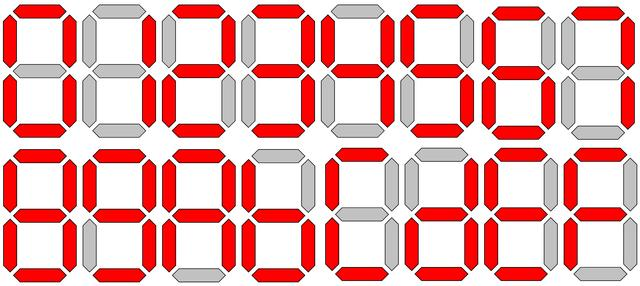
\includegraphics[width=15cm]{pictures/7seg.jpg}}
\end{center}

\subsubsection{meow}
miaounyanmeowmjau

\section{ALU}
\subsection{nyan}
\subsubsection{meow}
\subsubsubsection{mjau}
miaounyanmeowmjau

\section{Banc de registres}
\subsection{nyan}
\subsubsection{meow}
\subsubsubsection{mjau}
miaounyanmeowmjau

\section{Usage de la documentation ARM}
\subsection{nyan}
\subsubsection{meow}
\subsubsubsection{mjau}
miaounyanmeowmjau

\end{document}
